% Important note:
% Chapter heading images should have a 2:1 width:height ratio,
% e.g. 920px width and 460px height.
%
%%%%%%%%%%%%%%%%%%%%%%%%%%%%%%%%%%%%%%%%%

%----------------------------------------------------------------------------------------
%	PACKAGES AND OTHER DOCUMENT CONFIGURATIONS
%----------------------------------------------------------------------------------------

\documentclass[openany,14pt,fleqn]{book} % Default font size and left-justified equations
%openany is used to have the book style but having no blank pages in between chapitre


\usepackage[top=3cm,bottom=3cm,left=3.2cm,right=3.2cm,headsep=5pt,letterpaper]{geometry} % Page margins

\usepackage{xcolor} % Required for specifying colors by name
\definecolor{ocre}{RGB}{52,177,201} % Define the orange color used for highlighting throughout the book

% Font Settings
\usepackage{avant} % Use the Avantgarde font for headings
%\usepackage{times} % Use the Times font for headings
\usepackage{mathptmx} % Use the Adobe Times Roman as the default text font together with math symbols from the Sym­bol, Chancery and Com­puter Modern fonts




%header and footer
\usepackage{wrapfig}
\usepackage{fancyhdr}
\pagestyle{fancy}
\fancyhead{}
\fancyfoot{}
\fancyfoot[R]{\thepage}
\renewcommand{\headrulewidth}{1pt}
\renewcommand{\footrulewidth}{1pt}

\usepackage{microtype} % Slightly tweak font spacing for aesthetics
\usepackage[utf8]{inputenc} % Required for including letters with accents
\usepackage[T1]{fontenc} % Use 8-bit encoding that has 256 glyphs
\usepackage{listings}
\usepackage{etoolbox} %change chapter caracteristics
\makeatletter

%\documentclass[oneside]{book}



%\patchcmd{\chapter}{\cleardoublepage\else\clearpage\fi}{}{}{}
\makeatother
%%configuration de listings
\lstset{
language=Python,
basicstyle=\ttfamily\small, %
identifierstyle=\color{red}, %
keywordstyle=\color{blue}, %
stringstyle=\color{black!60}, %
commentstyle=\it\color{green!95!yellow!1}, %
columns=flexible, %
tabsize=2, %
extendedchars=true, %
showspaces=false, %
showstringspaces=false, %
numbers=left, %
numberstyle=\tiny, %
breaklines=true, %
breakautoindent=true, %
captionpos=b
}
\newsavebox{\BBbox}
\newenvironment{DDbox}[1]{
\begin{lrbox}{\BBbox}\begin{minipage}{\linewidth}}
{\end{minipage}\end{lrbox}\noindent\colorbox{Zgris}{\usebox{\BBbox}} \\
[.5cm]}
% Bibliography
\usepackage[style=numeric-verb,defernumbers=true,sorting=nyt,sortcites=true,autopunct=true,autolang=hyphen,hyperref=false,abbreviate=false,backref=true,backend=biber]{biblatex}
\addbibresource{bibliography.bib} % BibTeX bibliography file
\defbibheading{Source:}{}


%----------------------------------------------------------------------------------------
%	VARIOUS REQUIRED PACKAGES
%----------------------------------------------------------------------------------------

\usepackage{titlesec} % Allows customization of titles

\usepackage{graphicx} % Required for including pictures
\graphicspath{{Pictures/}} % Specifies the directory where pictures are stored

\usepackage{lipsum} % Inserts dummy text

\usepackage{tikz} % Required for drawing custom shapes

\usepackage[english]{babel} % English language/hyphenation

\usepackage{enumitem} % Customize lists
\setlist{nolistsep} % Reduce spacing between bullet points and numbered lists

\usepackage{booktabs} % Required for nicer horizontal rules in tables

\usepackage{eso-pic} % Required for specifying an image background in the title page

%----------------------------------------------------------------------------------------
%	MAIN TABLE OF CONTENTS
%----------------------------------------------------------------------------------------

\usepackage{titletoc} % Required for manipulating the table of contents

\contentsmargin{0cm} % Removes the default margin
% Chapter text styling
\titlecontents{chapter}[1.25cm] % Indentation
{\addvspace{15pt}\large\sffamily\bfseries} % Spacing and font options for chapters
{\color{ocre!60}\contentslabel[\Large\thecontentslabel]{1.25cm}\color{ocre}} % Chapter number
{}  
{\color{ocre!60}\normalsize\sffamily\bfseries\;\titlerule*[.5pc]{.}\;\thecontentspage} % Page number
% Section text styling
\titlecontents{section}[1.25cm] % Indentation
{\addvspace{5pt}\sffamily\bfseries} % Spacing and font options for sections
{\contentslabel[\thecontentslabel]{1.25cm}} % Section number
{}
{\sffamily\hfill\color{black}\thecontentspage} % Page number
[]
% Subsection text styling
\titlecontents{subsection}[1.25cm] % Indentation
{\addvspace{1pt}\sffamily\small} % Spacing and font options for subsections
{\contentslabel[\thecontentslabel]{1.25cm}} % Subsection number
{}
{\sffamily\;\titlerule*[.5pc]{.}\;\thecontentspage} % Page number
[] 

%----------------------------------------------------------------------------------------
%	MINI TABLE OF CONTENTS IN CHAPTER HEADS
%----------------------------------------------------------------------------------------

% Section text styling
\titlecontents{lsection}[0em] % Indendating
{\footnotesize\sffamily} % Font settings
{}
{}
{}

% Subsection text styling
\titlecontents{lsubsection}[.5em] % Indentation
{\normalfont\footnotesize\sffamily} % Font settings
{}
{}
{}
 
%----------------------------------------------------------------------------------------
%	PAGE HEADERS
%----------------------------------------------------------------------------------------

\usepackage{fancyhdr} % Required for header and footer configuration

\pagestyle{fancy}
\renewcommand{\chaptermark}[1]{\markboth{\sffamily\normalsize\bfseries\chaptername\ \thechapter.\ #1}{}} % Chapter text font settings
\renewcommand{\sectionmark}[1]{\markright{\sffamily\normalsize\thesection\hspace{5pt}#1}{}} % Section text font settings
\fancyhf{} \fancyhead[LE,RO]{\sffamily\normalsize\thepage} % Font setting for the page number in the header
\fancyhead[LO]{\rightmark} % Print the nearest section name on the left side of odd pages
\fancyhead[RE]{\leftmark} % Print the current chapter name on the right side of even pages
\renewcommand{\headrulewidth}{0.5pt} % Width of the rule under the header
\addtolength{\headheight}{2.5pt} % Increase the spacing around the header slightly
\renewcommand{\footrulewidth}{1pt} % Removes the rule in the footer
\fancypagestyle{plain}{\fancyhead{}\renewcommand{\headrulewidth}{1pt}} % Style for when a plain pagestyle is specified

% Removes the header from odd empty pages at the end of chapters
\makeatletter
\renewcommand{\cleardoublepage}{
\clearpage\ifodd\c@page\else
\hbox{}
\vspace*{\fill}
\thispagestyle{fancy}
\newpage
\fi}

%----------------------------------------------------------------------------------------
%	THEOREM STYLES
%----------------------------------------------------------------------------------------

\usepackage{amsmath,amsfonts,amssymb,amsthm} % For math equations, theorems, symbols, etc

\newcommand{\intoo}[2]{\mathopen{]}#1\,;#2\mathclose{[}}
\newcommand{\ud}{\mathop{\mathrm{{}d}}\mathopen{}}
\newcommand{\intff}[2]{\mathopen{[}#1\,;#2\mathclose{]}}
\newtheorem{notation}{Notation}[chapter]

%%%%%%%%%%%%%%%%%%%%%%%%%%%%%%%%%%%%%%%%%%%%%%%%%%%%%%%%%%%%%%%%%%%%%%%%%%%
%%%%%%%%%%%%%%%%%%%% dedicated to boxed/framed environements %%%%%%%%%%%%%%
%%%%%%%%%%%%%%%%%%%%%%%%%%%%%%%%%%%%%%%%%%%%%%%%%%%%%%%%%%%%%%%%%%%%%%%%%%%
\newtheoremstyle{ocrenumbox}% % Theorem style name
{0pt}% Space above
{0pt}% Space below
{\normalfont}% % Body font
{}% Indent amount
{\small\bf\sffamily\color{ocre}}% % Theorem head font
{\;}% Punctuation after theorem head
{0.25em}% Space after theorem head
{\small\sffamily\color{ocre}\thmname{#1}\nobreakspace\thmnumber{\@ifnotempty{#1}{}\@upn{#2}}% Theorem text (e.g. Theorem 2.1)
\thmnote{\nobreakspace\the\thm@notefont\sffamily\bfseries\color{black}---\nobreakspace#3.}} % Optional theorem note
\renewcommand{\qedsymbol}{$\blacksquare$}% Optional qed square

\newtheoremstyle{blacknumex}% Theorem style name
{5pt}% Space above
{5pt}% Space below
{\normalfont}% Body font
{} % Indent amount
{\small\bf\sffamily}% Theorem head font
{\;}% Punctuation after theorem head
{0.25em}% Space after theorem head
{\small\sffamily{\tiny\ensuremath{\blacksquare}}\nobreakspace\thmname{#1}\nobreakspace\thmnumber{\@ifnotempty{#1}{}\@upn{#2}}% Theorem text (e.g. Theorem 2.1)
\thmnote{\nobreakspace\the\thm@notefont\sffamily\bfseries---\nobreakspace#3.}}% Optional theorem note

\newtheoremstyle{blacknumbox} % Theorem style name
{0pt}% Space above
{0pt}% Space below
{\normalfont}% Body font
{}% Indent amount
{\small\bf\sffamily}% Theorem head font
{\;}% Punctuation after theorem head
{0.25em}% Space after theorem head
{\small\sffamily\thmname{#1}\nobreakspace\thmnumber{\@ifnotempty{#1}{}\@upn{#2}}% Theorem text (e.g. Theorem 2.1)
\thmnote{\nobreakspace\the\thm@notefont\sffamily\bfseries---\nobreakspace#3.}}% Optional theorem note

%%%%%%%%%%%%%%%%%%%%%%%%%%%%%%%%%%%%%%%%%%%%%%%%%%%%%%%%%%%%%%%%%%%%%%%%%%%
%%%%%%%%%%%%% dedicated to non-boxed/non-framed environements %%%%%%%%%%%%%
%%%%%%%%%%%%%%%%%%%%%%%%%%%%%%%%%%%%%%%%%%%%%%%%%%%%%%%%%%%%%%%%%%%%%%%%%%%
\newtheoremstyle{ocrenum}% % Theorem style name
{5pt}% Space above
{5pt}% Space below
{\normalfont}% % Body font
{}% Indent amount
{\small\bf\sffamily\color{ocre}}% % Theorem head font
{\;}% Punctuation after theorem head
{0.25em}% Space after theorem head
{\small\sffamily\color{ocre}\thmname{#1}\nobreakspace\thmnumber{\@ifnotempty{#1}{}\@upn{#2}}% Theorem text (e.g. Theorem 2.1)
\thmnote{\nobreakspace\the\thm@notefont\sffamily\bfseries\color{black}---\nobreakspace#3.}} % Optional theorem note
\renewcommand{\qedsymbol}{$\blacksquare$}% Optional qed square
\makeatother

% Defines the theorem text style for each type of theorem to one of the three styles above
\newcounter{dummy} 
\numberwithin{dummy}{section}
\theoremstyle{ocrenumbox}
\newtheorem{theoremeT}[dummy]{Theorem}
\newtheorem{problem}{Problem}[chapter]
\newtheorem{exerciseT}{Exercise}[chapter]
\theoremstyle{blacknumex}
\newtheorem{exampleT}{Example}[chapter]
\theoremstyle{blacknumbox}
\newtheorem{vocabulary}{Vocabulary}[chapter]
\newtheorem{definitionT}{Definition}[section]
\newtheorem{corollaryT}[dummy]{Corollary}
\theoremstyle{ocrenum}
\newtheorem{proposition}[dummy]{Proposition}

%----------------------------------------------------------------------------------------
%	DEFINITION OF COLORED BOXES
%----------------------------------------------------------------------------------------

\RequirePackage[framemethod=default]{mdframed} % Required for creating the theorem, definition, exercise and corollary boxes

% Theorem box
\newmdenv[skipabove=7pt,
skipbelow=7pt,
backgroundcolor=black!5,
linecolor=ocre,
innerleftmargin=5pt,
innerrightmargin=5pt,
innertopmargin=5pt,
leftmargin=0cm,
rightmargin=0cm,
innerbottommargin=5pt]{tBox}

% Exercise box	  
\newmdenv[skipabove=7pt,
skipbelow=7pt,
rightline=false,
leftline=true,
topline=false,
bottomline=false,
backgroundcolor=ocre!10,
linecolor=ocre,
innerleftmargin=5pt,
innerrightmargin=5pt,
innertopmargin=5pt,
innerbottommargin=5pt,
leftmargin=0cm,
rightmargin=0cm,
linewidth=4pt]{eBox}	

% Definition box
\newmdenv[skipabove=7pt,
skipbelow=7pt,
rightline=false,
leftline=true,
topline=false,
bottomline=false,
linecolor=ocre,
innerleftmargin=5pt,
innerrightmargin=5pt,
innertopmargin=0pt,
leftmargin=0cm,
rightmargin=0cm,
linewidth=4pt,
innerbottommargin=0pt]{dBox}	

% Corollary box
\newmdenv[skipabove=7pt,
skipbelow=7pt,
rightline=false,
leftline=true,
topline=false,
bottomline=false,
linecolor=gray,
backgroundcolor=black!5,
innerleftmargin=5pt,
innerrightmargin=5pt,
innertopmargin=5pt,
leftmargin=0cm,
rightmargin=0cm,
linewidth=4pt,
innerbottommargin=5pt]{cBox}

% Creates an environment for each type of theorem and assigns it a theorem text style from the "Theorem Styles" section above and a colored box from above
\newenvironment{theorem}{\begin{tBox}\begin{theoremeT}}{\end{theoremeT}\end{tBox}}
\newenvironment{exercise}{\begin{eBox}\begin{exerciseT}}{\hfill{\color{ocre}\tiny\ensuremath{\blacksquare}}\end{exerciseT}\end{eBox}}				  
\newenvironment{definition}{\begin{dBox}\begin{definitionT}}{\end{definitionT}\end{dBox}}	
\newenvironment{example}{\begin{exampleT}}{\hfill{\tiny\ensuremath{\blacksquare}}\end{exampleT}}		
\newenvironment{corollary}{\begin{cBox}\begin{corollaryT}}{\end{corollaryT}\end{cBox}}	

%----------------------------------------------------------------------------------------
%	REMARK ENVIRONMENT
%----------------------------------------------------------------------------------------

\newenvironment{remark}{\par\vspace{10pt}\small % Vertical white space above the remark and smaller font size
\begin{list}{}{
\leftmargin=35pt % Indentation on the left
\rightmargin=25pt}\item\ignorespaces % Indentation on the right
\makebox[-2.5pt]{\begin{tikzpicture}[overlay]
\node[draw=ocre!60,line width=1pt,circle,fill=ocre!25,font=\sffamily\bfseries,inner sep=2pt,outer sep=0pt] at (-15pt,0pt){\textcolor{ocre}{R}};\end{tikzpicture}} % Orange R in a circle
\advance\baselineskip -1pt}{\end{list}\vskip5pt} % Tighter line spacing and white space after remark

%----------------------------------------------------------------------------------------
%	SECTION NUMBERING IN THE MARGIN
%----------------------------------------------------------------------------------------

\makeatletter
\renewcommand{\@seccntformat}[1]{\llap{\textcolor{ocre}{\csname the#1\endcsname}\hspace{1em}}}                    
\renewcommand{\section}{\@startsection{section}{1}{\z@}
{-4ex \@plus -1ex \@minus -.4ex}
{1ex \@plus.2ex }
{\normalfont\large\sffamily\bfseries}}
\renewcommand{\subsection}{\@startsection {subsection}{2}{\z@}
{-3ex \@plus -0.1ex \@minus -.4ex}
{0.5ex \@plus.2ex }
{\normalfont\sffamily\bfseries}}
\renewcommand{\subsubsection}{\@startsection {subsubsection}{3}{\z@}
{-2ex \@plus -0.1ex \@minus -.2ex}
{.2ex \@plus.2ex }
{\normalfont\small\sffamily\bfseries}}                        
\renewcommand\paragraph{\@startsection{paragraph}{4}{\z@}
{-2ex \@plus-.2ex \@minus .2ex}
{.1ex}
{\normalfont\small\sffamily\bfseries}}

%----------------------------------------------------------------------------------------
%	HYPERLINKS IN THE DOCUMENTS
%----------------------------------------------------------------------------------------

% For an unclear reason, the package should be loaded now and not later
\usepackage{hyperref}
\hypersetup{hidelinks,backref=true,pagebackref=true,hyperindex=true,colorlinks=false,breaklinks=true,urlcolor= ocre,bookmarks=true,bookmarksopen=false,pdftitle={Title},pdfauthor={Author}}

%----------------------------------------------------------------------------------------
%	CHAPTER HEADINGS
%----------------------------------------------------------------------------------------

% The set-up below should be (sadly) manually adapted to the overall margin page septup controlled by the geometry package loaded in the main.tex document. It is possible to implement below the dimensions used in the goemetry package (top,bottom,left,right)... TO BE DONE

\newcommand{\thechapterimage}{}
\newcommand{\chapterimage}[1]{\renewcommand{\thechapterimage}{#1}}

% Numbered chapters with mini tableofcontents
\def\thechapter{\arabic{chapter}}
\def\@makechapterhead#1{
\thispagestyle{fancy}
{\centering \normalfont\sffamily
\ifnum \c@secnumdepth >\m@ne
\if@mainmatter
\startcontents
\begin{tikzpicture}[remember picture,overlay]
\node at (current page.north west)
{\begin{tikzpicture}[remember picture,overlay]
\node[anchor=north west,inner sep=0pt] at (0,0) {\includegraphics[width=\paperwidth]{\thechapterimage}};
%%%%%%%%%%%%%%%%%%%%%%%%%%%%%%%%%%%%%%%%%%%%%%%%%%%%%%%%%%%%%%%%%%%%%%%%%%%%%%%%%%%%%
% Commenting the 3 lines below removes the small contents box in the chapter heading
%\fill[color=ocre!10!white,opacity=.6] (1cm,0) rectangle (8cm,-7cm);
%\node[anchor=north west] at (1.1cm,.35cm) {\parbox[t][8cm][t]{6.5cm}{\huge\bfseries\flushleft \printcontents{l}{1}{\setcounter{tocdepth}{2}}}};
\draw[anchor=west] (5cm,-9cm) node [rounded corners=20pt,fill=ocre!10!white,text opacity=1,draw=ocre,draw opacity=1,line width=1.5pt,fill opacity=.6,inner sep=12pt]{\huge\sffamily\bfseries\textcolor{black}{\thechapter. #1\strut\makebox[22cm]{}}};
%%%%%%%%%%%%%%%%%%%%%%%%%%%%%%%%%%%%%%%%%%%%%%%%%%%%%%%%%%%%%%%%%%%%%%%%%%%%%%%%%%%%%
\end{tikzpicture}};
\end{tikzpicture}}
\par\vspace*{230\p@}
\fi
\fi}

% Unnumbered chapters without mini tableofcontents (could be added though) 
\def\@makeschapterhead#1{
\thispagestyle{empty}
{\centering \normalfont\sffamily
\ifnum \c@secnumdepth >\m@ne
\if@mainmatter
\begin{tikzpicture}[remember picture,overlay]
\node at (current page.north west)
{\begin{tikzpicture}[remember picture,overlay]
\node[anchor=north west,inner sep=0pt] at (0,0) {\includegraphics[width=\paperwidth]{\thechapterimage}};
\draw[anchor=west] (5cm,-9cm) node [rounded corners=20pt,fill=ocre!10!white,fill opacity=.6,inner sep=12pt,text opacity=1,draw=ocre,draw opacity=1,line width=1.5pt]{\huge\sffamily\bfseries\textcolor{black}{#1\strut\makebox[22cm]{}}};
\end{tikzpicture}};
\end{tikzpicture}}
\par\vspace*{230\p@}
\fi
\fi
}
\makeatother % Insert the commands.tex file which contains the majority of the structure behind the template
\setlength{\parindent}{0em}
\begin{document}

%----------------------------------------------------------------------------------------
%	TITLE PAGE
%----------------------------------------------------------------------------------------

\begingroup
\thispagestyle{empty}
\AddToShipoutPicture*{\put(0,0){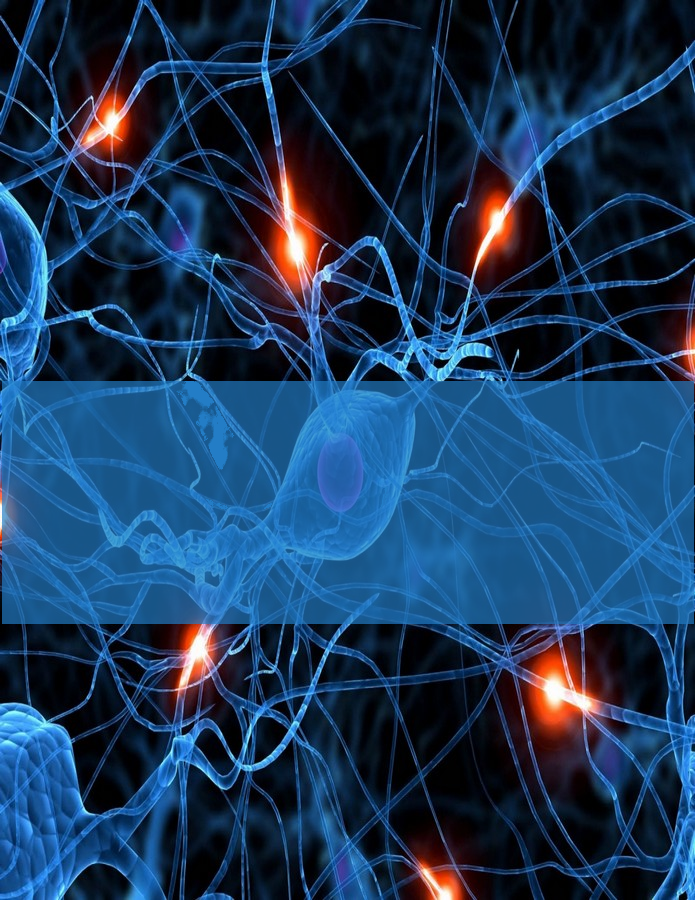
\includegraphics[scale=1.25]{try}}} % Image background
\centering
\vspace*{5cm}
\par\normalfont\fontsize{35}{35}\sffamily\selectfont
\textbf{réseaux neuronaux artificiels}\\
{\LARGE l'apprentissage d'une machine}\par % Book title
\vspace*{1cm}
{\Huge Da Silva Gameiro Henrique}\par % Author name
\endgroup


%----------------------------------------------------------------------------------------
%	TABLE OF CONTENTS
%----------------------------------------------------------------------------------------
\renewcommand{\contentsname}{Table des matières}
\chapterimage{Pictures/NN.jpeg} % Table of contents heading image

\thispagestyle{empty} % No headers
\setcounter{page}{1}
\tableofcontents % Print the table of contents itself
\pagenumbering{arabic}
%\setcounter{page}{1}


\thispagestyle{fancy}
\fancyhead{}
\fancyfoot{}
\fancyfoot[R]{\thepage}
%\fancyhead[LO]{\rightmark} % Print the nearest section name on the left side of odd pages
\fancyhead[L]{\leftmark} % check fancyhead on google
\renewcommand{\headrulewidth}{1pt}
\renewcommand{\footrulewidth}{0pt} % Print headers again\\

%----------------------------------------------------------------------------------------
%	CHAPTER 1
%----------------------------------------------------------------------------------------

%\break \chapterimage{head2.png} % Chapter heading image


\chapter{Introduction}
\section{Définition du Machine learning}
Le machine learning ou apprentissage automatique est un sous-ensemble de l'intelligence artificielle(A.I) selon l'encyclopédie Larousse, l'A.I. se définit comme  «l'ensemble de théories et de techniques mises en œuvre en vue de réaliser des machines capables de simuler l'intelligence »\cite{Wikipedia_def}. Le machine learning fait donc parti de cette ensemble.\\
Comme ce domaine a beaucoup évolué au cours des années, mais l'idée était déjà définie en 1959 par Arthur Samuel:«Le machine learning est le domaine d'étude qui donne à l'ordinateur la capacité d'apprendre sans être explicitement programmé»(traduit de l'anglais).\\
Tom Mitchell définit aussi l'apprentissage d'un algorithme de machine learning en 1998 «On programme un algorithme informatique pour qu'il apprenne d'une une expérience E selon une certaine fonction T(task) et une mesure de performance P, si sa performance aux fonctions T, mesurée par P, augmente avec l'expérience E »\\ 
On peut illustrer cette définition par un exemple: dans le  cas d'un algorithme qui apprendrait à jouer à un jeu, le E serait l'expérience d'avoir joué ou vu quelqu'un joué, le T serais la fonction de joueur à ce jeu et P la probabilité de gagner une partie. Ces notions sont présente aussi pour parler des différents concepts dans un réseau de neurone, mais avec un nom différent.\\ 
Le E sera l'ensemble d'entraînement D et le P sera l'erreur ou le delta entre ce qu'on cherche à obtenir et ce qu'on prédit.\cite{Coursera}

\section{Types d'apprentissage}
Pour résoudre un problème de Machine learning, il faut d'abord déterminer le type d'algorithme ou type de réseau de neurone.\\
Il existe 2 grandes catégorie d'apprentissages: \underline{supervisé} et \underline{non-supervisé}\\ \break
Dans un algorithme d'apprentissage supervisé, nous utilisons des exemples d'entraînement avec un ensemble de départ et d'arrivée. A partir de ces exemples, l'algorithme va apprendre; c'est comme si par de la "data" nous apprenions à la machine à par exemple reconnaître des images.\\
En apprentissage supervisé, il existe encore des sous-catégories(parfois combinés):\\
Tous d'abord, les algorithmes de \underline{régression}: ceux-ci prédisent une valeur futur en continu à partir de résultats passés comme un prix d'un appartement par exemple.\\
La 2ème catégorie est la \underline{classification}: dans ces algorithmes, les valeurs d'ensemble d'arrivées sont des \underline{classes} comme des chiffre ou un type d'image. Le but est que l’algorithme trouve la classe correspondante à un élément de l’ensemble de départ. Pour ce faire, on utilise une fonction linéaire ou quadratique pour faire une séparation entre classes.\\ \break
Dans les problèmes d'apprentissage non-supervisé, il n'y a pas d'ensemble d'arrivée dans nos exemples d’entraînement: nous ne connaissons pas à l'avance le résultat que doit a obtenir l'algorithme et on peut ainsi résoudre des problèmes sans savoir à quoi le résultat devrait ressembler.\\
Leurs utilisations est très vaste les plus basiques sont exemple de trouver des liens entre des éléments de notre data et les grouper comme le fait d'identifier des groupes d'amis utilisé par facebook ou lorsqu'on fait une recherche sur un moteur de recherche, trouver des sites en liens avec ce qu'on recherche. Justement, le terme utilisé pour évaluer l'efficacité de ce type d'algorithme, c'est-à-dire le degrés de ressemblance entre ce qu'on cherche à obtenir et ce qu'on obtient s'appelle \underline{"fitness"}.\cite{Wikipedia_def}
\section{L'histoire du machine learning en bref:mettre des images de personnes}
Aussi surprenant que cela puisse paraître, les premiers réseaux de neurones artificiels ont été théorisés avant la création des premiers ordinateurs. En effet, le moteur premier de l'avancer du machine learning a été les neurosciences dans un premier temps(est les toujours en partie).\\ Ce sont les neuroscientifiques Walter Pitts et Warren McCulloch qui ont eu l'idée d'appliquer les mathématique aux réseaux de neurones pour reproduire leur fonctionnement dans leur travail de séminaire “A Logical Calculus of Ideas Immanent in Nervous Activity”.Leur idée est de reproduire la pensée avec des calculs mathématiques.\\
Alan Turing ,théoricien de l'ordinateur et de la programmation, voyait déjà, en 1950, l'impact considérable que pourrait avoir le machine learning dans le futur. Il a créé aussi le célèbre test de Turing établissant un seuil où il considère que l'algorithme est assez intelligent pour penser comme une humain. Le test consiste en une simple conversation entre un humain et une intelligence artificielle puis avec un humain. L'intelligence réussit le test si l'humain ne peux pas discerner lequel des deux est un ordinateur.Certains pensent que ce test a déjà été passé aujourd'hui par certains algorithmes, mais c'est un sujet très débattu(notamment avec la démonstration de google duplex).\\ \\
En 1952, Arthur Samuel crée un programme jouant aux dames. Ce dernier apprend par lui-même et devient meilleur de partie en partie selon ses erreurs. Cette exemple a mis en évidence un des principes du machine learning qui est l'apprentissage automatique de l'intelligence.\\
Le premier perceptron est créé,en 1957, par Frank Rosenblatt. C'est la base des réseaux de neurones artificiels encore aujourd'hui. Il consiste en un seul neurone, mais possède déjà les bases d'un réseau de neurone. Cette découverte a produit un grand engouement pour le domaine. Cependant, les limitations du perceptron va étouffer cette élan\footnote{il y a eu 2 périodes appelées "AI winter"(1974-80 et 1987-93) durant lesquelles l'engouement pour l'intelligence était moindre à cause de blocages technologique} et il a fallu attendre d'autre découvertes pour que le machine learning prenne la place qu'il a aujourd'hui.\\
La théorie va passer à la pratique en 1965 avec Alexey Ivakhnenko qui va créer le premier réseau artificiel fonctionnel. Il a aussi développé des réseaux à plusieurs couches jusqu'à 8.\\
En 1980, le premier réseau à convolution(CNN\footnote{cf. chapitre sur les CNN}) est inventé ,selon le cortex des animaux, pour pouvoir faire de la reconnaissance d'image.\\
En 1982 est inventé le premier réseau à neurones récursifs par John Hopfield. Les neurones de ce type d'algorithmes sont proches des neurones biologiques puisqu'ils ont une plus grand mémoire que ceux des autre type de réseaux artificiels.\\
David Rumelhart, Ronald J. Williams et plus particulièrement Geoffrey Hinton ont dévelopé la backpropagation en 1986. Cette découverte a permis d'augmenter considérablement la performance des réseaux et a été un catalyseur pour le machine learning.\\
En 1989, le français Yann LeCun a mis au point un algorithme permettant de lire des chiffres écrits à la main en utilisant les CNN et la backpropagation. Cette application deviendra un étalon de mesure de la performance d'un réseau.\\
Dans cette même période, le Q-learning (plus tard apprentissage par renforcement) est découvert par Christopher Watkins. Le principe est de corriger le réseau par récompenses lorsque le réseau fait un bon choix. Le but est donc de prendre des actions maximisant la récompense plutôt que de minimiser l'erreur.\cite{history,wiki_history}






---






%----------------------------------------------------------------------------------------
%	CHAPTER 2
%----------------------------------------------------------------------------------------
%\chapterimage{band1.png}

\chapter{Premier modèle: le perceptron}
\section{Principe général du perceptron}\index{First ideas}
Le principe du perceptron est de modéliser une décision par une fonction linéaire et un seuil(Threshold en anglais) pour pouvoir classer des entrées $x_1,x_2,\dots,x_n$ et qu'elle formule une hypothèse hw(x) qui doit s'approcher d'une sortie yt voulue\cite{3Blue1Brown,Hugo_Larochelle4,giant_neural}

\begin{figure}[h]
    \centering
    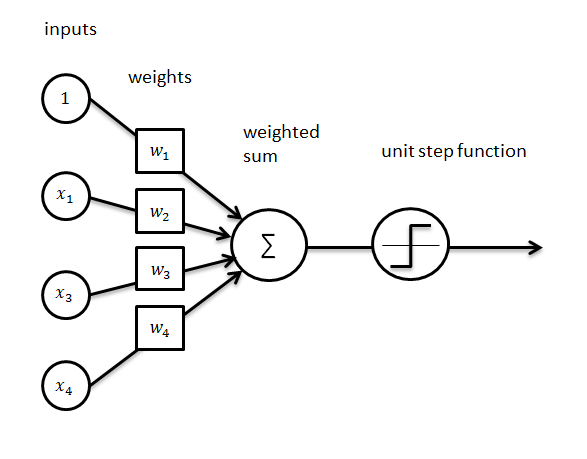
\includegraphics[width=0.77\textwidth]{Pictures/perceptron.png}
    \caption{perceptron }
    \label{fig:awesome_image}
\end{figure}
\begin{equation}                                                                                                hw(x) = Threshold(W\cdot x)\end{equation}
où $Threshold(z) = 1$  si $z \geq$ 0, 
sinon $Threshold(z) = 0$ : c'est la prise de décision, l'activation d'un neurone.\\\\ L'activation, dans le perceptron, est une fonction linéaire. On peut donc se représenter le fonctionnement d'un perceptron par une fonction linéaire c'est à dire une droite : celle-ci sépare les éléments en entrée en 2 classes. \newline Le perceptron est donc un classificateur linéaire qui ne peut traiter que les problèmes transformable linéairement(cf.chapite 3.1).\\ Plus généralement, l'activation est en fait inspiré du cerveau. Un neurone biologique ne s'allume que si il reçoit un signal électrique dépassant un certains seuil. Pour notre perceptron, c'est exactement ce prinicipe qui est utilisé.
\begin{figure}[h]
\centering
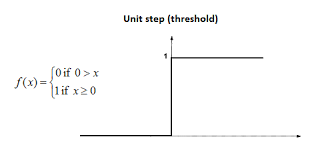
\includegraphics[width=0.7\textwidth]{Pictures/t_l_chargement.png}
\caption{fonction threshold}
\end{figure}
z correspond au produit matricielle des vecteurs-colonnes entrés($x1,x2,\cdots xn$) et poids($w1,w2,\cdots wn$). Le poids d'une connexion,appelé aussi poids synaptique, représente l'influence d'une connexion sur un neurone, c'est-à-dire la valeur d'un input xn par rapport à l'output y. On pourrait représenter ceci dans un exemple concret pour prendre une décision:imaginons qu'on doive décider d’assister à un concert on pourrait prendre par exemple 4 facteurs qui influencerait notre décision:x1 le groupe qui joue à ce concert, x2 le prix du billet, x3 les personnes qui vont nous accompagner et x4 la date du concert. Imaginons que le groupe qui joue nous importe peu(w1),que nous somme en difficulté financière(w2),que nous voulons absolument y aller en grand nombre(w3) et que nous sommes en vacances. Nous remarquons que certaines variables ont une plus grand variables :x2 et x3 sont plus important et par conséquent la valeur de w2 et w3 en saura d'autant plus grand que l'impact de x2 et x3 sur notre décision.\newline\smallbreak 
Le but de l’algorithme est de trouver les bonnes valeurs pour le vecteur de poids W: c'est le paramètre, ce qui va changer au cours des entraînements.
On utilise cependant aussi un biais b qui sert à faire varier le seuil pour trouver le bon,le biais représente la difficulté d'un neurone à s'activer,doit-il s'activer fréquemment ?(comme un neurone biologique), plus il est élevé,plus un neurones s'active facilement et, au contraire, plus il tend vers les négatifs plus l'activation du neurone sera difficile, le bias peut être considéré comme 1 neurone ajouté en plus à chaque couche non influencé par la couche précédente : \newline
$Threshold(z)=1$ si $z\geq-b\Rightarrow Threshold = -b$ va donc aussi varier au cours de l'entraînement
\begin{figure}[h]
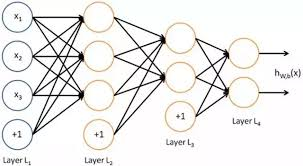
\includegraphics[width=0.7\textwidth]{Pictures/biais.jpg}
\caption{réseau de neurones avec biais}
\begin{remark} le +1 représente le biais
\end{remark}
\end{figure} cf https://www.quora.com/What-is-bias-in-artificial-neural-network
\section{Algorithme d'apprentissage du perceptron}
L'algorithme d'apprentissage doit adapter les paramètres W et b pour faire en sorte que la prédiction hw(x) soit la bonne valeur pour l'ensemble d'entraînement.\newline\smallbreak
1) Pour chaque paire$(xt,yt)\in D$ (xt = input,yt = target output et D = ensemble d'entraînement):\newline
\begin{itemize}\item calculer $hw(xt)=Treshold(w\cdot xt+b)$\newline
\item si $yt\neq hw(xt)$:$wi\leftarrow wi+\eta (yt-hw(xt))\cdot xt,i$\newline \end{itemize}
2) Retourner à l'étape 1 (itération) jusqu'à ce qu'on atteigne un critère d'arrêt comme un nombre maximal d'itération ou un seuil d'erreur satisfaisant.\newline
-La mise à jour des poids est appelée la règle d'apprentissage du perceptron. Son obtention sera détaillé dans la suite du document.\newline
-Le coefficient $\eta$ est le taux d'apprentissage et est lié au gradient.\newline
Dans la pratique ce calcul ce fera sous la forme matricielle pour une plus grande efficacité:\newline\smallbreak
$\begin{pmatrix} x1\\x2\\\vdots\\xn\\\end{pmatrix}\bullet \begin{pmatrix} w1\\w2\\\vdots\\wn\\\end{pmatrix}+\begin{pmatrix}
b\\\end{pmatrix}=\begin{pmatrix}hw(x1)\\hw(x2)\\\vdots\\hw(xn)\\\end{pmatrix}\approx\begin{pmatrix} y1\\y2\\\vdots\\yn\\\end{pmatrix}$


\section{Exemple d'apprentissage du perceptron}
Ensemble d'entraînement D\cite{Hugo_Larochelle5} :
\begin{tabular}{ c | r  }
	$ xt$& $yt $\\ \hline
   $[2,0]$& 1 \\
   $[0,3]$& 0 \\
   $[3,0]$& 0 \\
   $[1,1]$& 1 \\
 	\end{tabular}\\ \\
\underline {initialisation des paramètres ex: $\eta =0.1,W=[0,0],b=0.5$:}\\ \\
\underline {1ère itération avec$(x1,y1)$:}\break
\begin{itemize}
\item $h(x1) = Threshold(W\cdot x1+b)=Threshold([0,0]\cdot [2,0] +0.5)=Threshold(0,5)=1:$\newline
\item $h(x1) = y1\Rightarrow:$pas de mise à jour de W et b\newline
\end{itemize}
\underline {2ème itération avec (x2,y2):} \break
\begin{itemize} 
\item -$h(x2)=Threshold(W\cdot x2+b)=Threshold(0.5)=1:$\newline
\item puisque $h(x2)\neq y2$,on met à jour W et b :\\ $w\leftarrow w+\eta (y2-h(x2))\cdot x2\leftrightarrow[0,0]+0.1 \cdot(0-1)\cdot [0,3]=[0,-0.3]$\\
$b\leftarrow b+\eta(y2-h(x2))\cdot 1 =0.5+0.1(0-1)=0.4$\newline
\end{itemize}
\underline {3ème itération avec$(x3,y3)$ et $W=[0,-0.3]$et b=0.4$:$}\break
\begin{itemize}
\item -$h(x3)=Threshold(W\cdot x3+b)=Threshold(0.4)=1$,puisque $h(x3)\neq y3$,mise à jour de W et b:\newline$w\leftarrow w+\eta(y-h(x3)\cdot x3\leftrightarrow[0,-0.3]+0.1(0-1)\cdot[3,0]
=[-0.3.-0.3]\newline
b\leftarrow 0.4+0.1(0-1)=0.3$\newline
\end{itemize}
\underline{4ème itération avec $(x4,y4) et W=[-0.3,-0.3], b=0,3$}\break
\begin{itemize}
\item -$h(x4) = Threshold(W\cdot x4+b) = Threshold(-0.3)=0$,puisque $h(x4)\neq y4$ mise à jour de W et b:\\
$w = [-0.2,-0,2]$\\
$b = 0.4$
\end{itemize}

$\cdots \rightarrow$itérations jusqu'au critère d'arrêt.
\section{Exemple d'utilistaion du perceptron avec des portes logiques}
Les portes logiques constituent la base d'un ordinateur : elles permettent d'effectuer des opérations ou instructions avec des bytes ayant deux états possibles (0 ou 1)















Fonctionne pour OR,... mais pas XOR pas lin sép. On doit utiliser un perceptron multicouche(MLP) avec 3 neurones ce qui va donner à plus grandes échelle un NN de type feed forward $\neq reccurent$ appellé réseau convultionnaire utilisé pour la reconnaissance d'image\\

\section{Algorithme de correction des poids et biais}
Trouver les bon paramètres consiste en un problème d'optimisation: trouver le minimum d'une \underline {erreur}. Cette erreur est la distance entre l'output ciblée et la prédiction:$delta=yt-hw(xt)$\begin{remark}Nb Cette distance est aussi souvent appelé coût ou encore perte\end{remark}
Cette fonction dépend des variables pour hx(xt):W et b, ce sont donc plus d'une variable qu'il faut minimiser et donc il faut considérer l'utilisation de \underline{la dérivée partielle} et \underline {le gradient} $\nabla$ .\\
Le gradient nous donne la direction de l'augmentation la plus grande de la fonction. Prendre $-\nabla$ avec un coefficient(le taux d'apprentissage $\eta$ )permet de diriger la fonction erreur vers un minimum local(pas forcément le bon) et ainsi de minimiser cette fonction. Ce processus est appelé descente de gradient.\\ \linebreak
En revanche, calculer le gradient pour tout l'ensemble d'entraînement et ensuite un gradient serait en vérité beaucoup trop long si l'ensemble d'entraînement est grand, car on devrait calculer la moyenne des dérivées surs tous les exemples d'entraînement. Pour cela, on utilise \underline{la descente de gradient stochastique} le but et de sélectionner quelques exemples d'entraînement aléatoirement pour obtenir un \underline {"mini-batch"} il s'avère que calculer le gradient moyen pour ce "mini-batch" revient à trouver une approximation proche de la vraie valeur du gradient.\newline Cette approximation ne pose pas de problème en machine learning car nous ne cherchons pas à avoir une réponse exact mais connaître une direction vers laquelle on veut que nos variables tendent.
Ensuite, après avoir une correction avec le 1er "mini-batch",on en prend un 2ème et ainsi de suite jusqu'à avoir utiliser tout les exemples d'entraînement. Toute cette procédure constitue ce qu'on appelle une"epoch" et donc ce processus de "mini-batch" recommence pour chaque "epoch",
La progression de l'erreur peut être représenté par une courbe appelé \underline {courbe d'apprentissage} c'est le taux d'erreur par itération.\\
\begin{figure}[h]
\centering
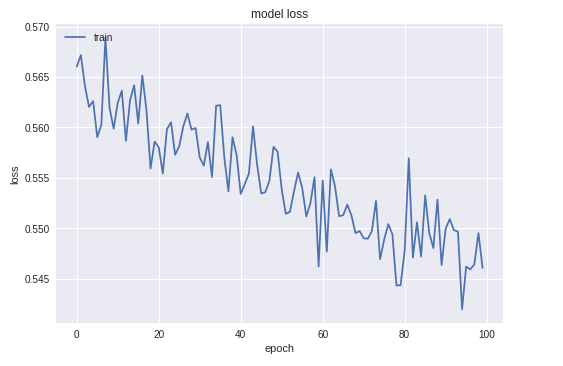
\includegraphics[width=0.7\textwidth]{Pictures/Courbe d'apprentissage.png}
\caption{courbe d'apprentissage}
\end{figure}
\section{Obtention de la règle d'apprentissage du perceptron}

On utilise le gradient avec les dérivées partielles pour avoir une direction de mise à jour des paramètres\cite{Hugo_Larochelle8,Hugo_Larochelle9}:\\
$$\nabla = \frac{\partial}{\partial wi} Loss(yt,hw(xt)) = \frac{\partial}{\partial wi}-(yt-hw(xt))\cdot w \cdot xt = -(yt-hw(xt))xt,i$$
Comme le gradient donne la direction d'augmentation la plus grande de la perte, on va dans la direction opposée $-\nabla$ pour la mise à jour des poids. A noter que pour la backporpagation, seule les dérivées partielles selon les poids sont nécessaires, alors le gradient consiste seulement en la dérivée partielle de la fonction selon les poids.  :\\
$$wi\Leftarrow wi- \eta \frac{\partial}{\partial wi} Loss(yt,hw(xt))\forall i$$
En remplaçant le gradient avec le gradient qu'on a obtenu plus haut on obtient la règle d'apprentissage du perceptron:\\
$$wi\leftarrow wi + \eta (yt-hw(xt))\cdot xt,i \forall i$$\\

\section{régression logistique(activation sigmoid}
Le problème d'utiliser la fonction Threshold comme activation est que cette fonction n'est pas dérivable partout, elle est discontinue; ceci peut mener à des approximations.\cite{Hugo_Larochelle10}\\ \break 
Il y a donc d'autre fonction d'activation est celui qui va nous intéresser dans ce chapitre est \underline{sigmoid}:
$$ \sigma(x) = \frac{1}{1+\exp ^- x}$$
\begin{figure}[h]
\centering
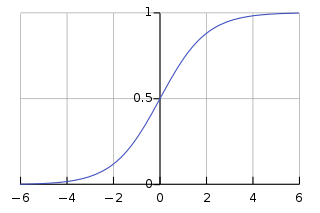
\includegraphics[width=0.5\textwidth]{Pictures/320px-Logistic-curve_svg.png}
\end{figure}\\
Cette fonction à l'avantage de ne pas être discontinue. Elle converti l'entrée x en probabilité\\
L'idée de ce système de classification est de se baser sur la probabilité d'appartenir à une classe:\\
$$p(y=1|x) = hw(x) = Sigmoid(w\cdot x) = \frac{1}{1+\exp ^{-w\cdot x}}$$
A partir de cette probabilité, l'algorithme choisit la classe la plus probable.
\chapter{Les réseaux de neurones artificiels (ou ANN pour artificial neural network)}
\section{problème des classificateurs linéaires à une couche}
Les perceptrons à une couche fonctionnent trés bien pour les problème dit \underline{séparable linéairement}, c'est-à-dire les cas où les différents objets regroupé en \underline classe(ex: pour les fonctions logique 0 est une classe et 1 une autre) puissent être séparés par une fonction linéaire comme c'est le cas pour les fonction logiques ET, OU, et même implique.\cite{Hugo_Larochelle11} 
\newline schéma:
\newline Cependant, ce même modèle du perceptron ne fonctionne pas pour des problèmes qui ne paraissent à première vue pas plus compliqué; c'est le cas pour XOR.
\newline En effet, la différence du où exckusif et qu'on ne puet pas séparer les classes d'objets par une droite : il n'est \underline{non-séparable linéairement} 
\newline schéma:
\newline Le perceprton de base ne peut donc par conséquent pas apprendre XOR,Ce problème est cependant fréquent. En effet, la plus part des problèmes ne sont pas séparable linéairement.
\newline
\section{les perceptrons multi-couches}
Pour résoudre des problèmes non-linéaires, une des première solutions trouvée a été de créer des perceptrons à plusieurs couches ou MLP(\textit{multi-layer perceptron})
\newline L'idée derrière ces systèmes et de transformer l'entrée pour la rendre linéairement séparable avec une première couche et ensuite une deuxième couche qui fonctionne comme les perceptrons vus précédemment.
\newline Pour le cas du XOR, une des solutions serait d'avoir 2 neurones sur la 1ère couche: un première qui va transformer l'entrée X1 par ET(x1,x2) et un 2ème neurone qui va transformer x2 par OU(x1,x2). Ainsi, le problème sera linéairement séparable
\newline
schéma:
\newline Dans ce modèle on a donc un neurone qui va apprendre OU un autre ET qui seront relié à autre neurone sur une 3ème couche qui va apprendre XOR ex code:







\ Ce processus encore assez primitif  d'utiliser plusieurs couches de neurones pour rendre le problème séparable linéairement est pourtant la base de ce qui va nous intéresser plus particulièrement dans ce travail à savoir les \underline{réseaux de neurones artificiels}
\section {définition d'un réseau de neurone à L couche}
Le but d'un réseau de neurone est, comme pour le perceptron, d'apprendre des poids pour pouvoir classer, mais les couches intermédiaires("hidden layer") permettent de rendre le problème linéairement séparable ou, plus basiquement, juxtaposer des couches de neurones permet d'avoir un corrélation plus évidente entre l'entrée et la sortie.\\
Par exemple, dans le cas de la reconnaissance de nombres, on peut imaginer que chaque couche décomposerait les nombres en parties et essayerait de reconnaître des paternes dans les pixels actifs pour pouvoir les faire correspondre à un nombre selon sa les parties constituant l'image d'entrée. Cependant, ce n'est pas ce que fait réellement l'algorithme, mais il suit ce principe.\\
Il existe plusieurs notations pour un réseau de neurones, l'une d'entre elle numérote les couches de haut en bas selon les couches. Les poids sont notés $w_{j,k}$(j et k représente les 2 neurones que la liaison relie), aj est l'activité dûn neurone j et inj l'activiét du neurone j avant l'activation :
\[ aj=Sigmoid(inj)\]\\
\underline{NB.}: $inj = z$
\underline{notations}:
j\\
k\\
\section{backpropagation ou rétropropagation des gradients/erreurs}
Dans le perceptron à une seule couche, calculer l'erreur de la dernière couche consistait en la différence entre la cible yt est notre prédiction hw(x).\\
Cependant, dans ce cas-ci il n'y a plus une seule couche et cette méthode ne fonctionne pas pour calculer l'erreur des neurones des couches cachées(ou hidden layer)\\
Pour cela on utilise la dérivée en chaîne(ou dérivée d'une fonction$f(g(x)) $),$$\frac{\partial f(x)}{\partial x} = \frac{\partial f(x)}{\partial g(x)}\cdot \frac{\partial g(x)}{\partial x}
\Rightarrow \frac{\partial f(x)}{\partial x} = \sum_{i} \frac{\partial f(x)}{\partial gi(x)}\cdot \frac{\partial gi(x)}{\partial x} $$ elle nous permet de calculer une dérivée à partir d'un résultat intermédiaire. Ainsi, On peut calculer la dérivée d'un neurone à une couche L à partir de la dérivée des neurones connectés à ce dernier à la couche suivante L+1.\cite{Hugo_Larochelle12}\\
Ce processus de retour en arrière s'appelle \underline{"backpropagation"}.\\
Elle constitue la 3ème étape de l'apprentissage et est un mouvement dans le sens contraire du "feed forward" et elle début par le calcul de l'erreur c'est-à-dire la différence entre le résultat ciblé et celui obtenu.\\
\\La backpropagation consiste donc à se servir de l'écart entre notre prédiction et le résultat ciblé et de propager cette erreur dans l'autre sens. Avec le poids des différents liens entre les neurones, on peut calculer l'erreur de chaque neurone(trouver le gradient) et ainsi mettre à jour les paramètres.\\
La dérivée partielle appliquée au NN donne la formule suivante: 
\[\frac{\partial Loss}{\partial inj} = \frac{\partial Loss}{\partial aj}\cdot \frac{\partial aj}{\partial inj} = (\sum_{k} \frac{\partial Loss}{\partial ink}\cdot \frac{\partial ink}{\partial aj})\cdot \frac{\partial aj}{inj} = (\sum_{k} \frac{\partial Loss}{\partial ink} \cdot w_{j,k})\cdot aj(1-aj) \]
\underline{remarques}:\\
-le j et k fait référence à la notation des neurones et des poids vue au-dessus: le j est le numéro d'un neurone à la couche L(couche actuelle) et k est le numéro du neurone relié au neurone j à la couche L+1(couche suivante)\\
-$aj = activation(inj)$ où $inj = W\cdot xn +b$ pour un j-ène neurone\\
- le premier terme entre parenthèse est la dérivée en chaîne de $\frac{\partial Loss}{\partial aj}$ celui-ci signifie qu'on itère à travers les neurone à la couche k(L+1)\\
- la dérivée partielle $\frac{\partial ink}{\partial aj} = wj,k$ et$\frac{\partial aj}{\partial inj} = aj(1-aj)$ soit la dérivée de la fonction sigmoid($\frac{df}{dx} = x(1-x)$)\\
-pour calculer l'erreur à la dernière couche, il peut être judicieux de mettre la différence au carré pour éviter les valeurs négatives. Ce calcul s'appelle(MSE\footnote{pour mean squared error traduit en erreur quadratique moyenne en français}), cependant on peut aussi utiliser la valeur absolu(à noter qu'il existe encore d'autre méthode pour calculer le delta).

\begin{figure}

\end{figure}
\section{mise à jour des paramètres dans un réseau de neurones}
Comme nous sommes toujours dans un problème d'optimisation, la mise à jour des paramètres pour le réseau de neurone se fait de la même façon en principe que le percerptron : on se sert des erreurs de chaque neurone calculé avec la backpropagation nous donnant la direction minimisant l'erreur de la fonction.
La formule générale est donc $$wi,j \leftarrow w_{i,j} +\alpha\cdot ai\cdot\Delta[j]$$.
$\Delta[j]$ est l'erreur pour chaque neurone j que nous avons vu ci-dessus avec la backpropagation c'est-à-dire pour rappel: $$ -\Delta[j] = \frac{\partial}{\partial inj}Loss(yt-hw(xt))$$ et $$ai = \frac{\partial}{\partial w_{i,j} \cdot inj}$$
La formule complète est donc: 
$$wi,j \leftarrow w_{i,j} -\alpha \cdot \frac{\partial}{\partial inj}Loss(yt-hw(xt)) \cdot \frac{\partial}{\partial w_{i,j} \cdot inj}$$
à savoir que $\frac{\partial}{\partial inj} Loss = sigmoid(z)(1-sigmoid(z))$  comme vu plus haut.


\section{exemple d'apprentissage d'un réseau de neurone avec backpropagation}
Nous allons reprendre la même donnée que pour le perceptron\\
donnée:\\ \\
\underline{propagation avant:}\\ \\
neurone $j_{3}: ak_{3}\footnote{pour rappel le neurone k est le neurone à la couche L+1 par rapport à j} = sigmoid(z\footnote{$z = \underset{j}{\Sigma} w_{j,k}\cdot aj$})=\sigma(2\cdot 2+0\cdot 1.5) = 0,982$\\
neurone $j_{4}: ak_{4} = sigmoid(z)=\sigma(2\cdot (-1)+0\cdot (1)) = $\\
neurone $j_{5}: ak_{5} = sigmoid(z)=\sigma((-2)\cdot 0,982+3\cdot (0,119)) = 0,167$\\
neurone $j_{6}: ak_{6} = sigmoid(z)=\sigma(1\cdot 0,982+2.5\cdot (0,119)) = 0,782$\\
neurone $j_{7}: ak_{7} = sigmoid(z)=\sigma((-2)\cdot 0,167+2\cdot (0,782)) = 0.773$\\ \\
\underline{backpropagation:}\\ \\
$\Delta_{j7} = y-a = 1-0,773 = 0,227\\
\Delta_{j6} = \sigma(inj)(1-\sigma(inj))\cdot \underset{k}{\Sigma}wj,k\cdot \Delta[k]\\$
\hspace*{0.4cm} $=0,782\cdot (1-0,782)\cdot 2\cdot 0,227 = 0,077\\
\Delta_{j5} = 0,167\cdot (1-0,167)\cdot -2\cdot 0,227 = -0,063\\
\Delta_{j4} = 0,119\cdot (1-0,119)\cdot(2,5\cdot 0,077+3\cdot (-0,063)) = 0,000366\\
\Delta_{j3} = 0,982\cdot (1-0,982)\cdot(1\cdot 0,077+(-2)\cdot (-0,063)) = 0,00358$\\ \\
\begin{figure}[h!]
\centering
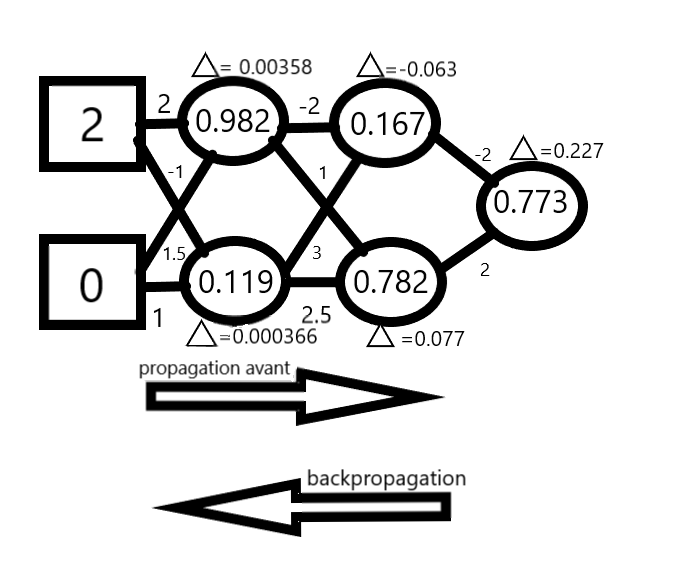
\includegraphics[width=0.7\textwidth]{Pictures/NNexemple.png}
\caption{exemple de réseau de neurones }
\end{figure}\\
\underline{mise à jour:}\\ \\
$w_{1,3}\leftarrow w_{i,j}+\alpha\cdot a_{i}\cdot\Delta[j] = 2+0,9\cdot 2\cdot 0,00358 = 2,0064 \\
w_{1,4}\leftarrow(-1)+0,9\cdot 2\cdot 0,000366 = -0,99934\\
w_{2,3}\leftarrow1,5+0,9\cdot 0\cdot 0,00358 = 1.5\\
w_{2,4}\leftarrow1+0,9\cdot 0\cdot 0,000366 = 1\\
w_{3,5}\leftarrow(-2)+0,9\cdot 0,982\cdot (-0,063) = -2,0556\\
w_{3,6}\leftarrow1+0,9\cdot 0,982\cdot 0,077 = 1,068\\
w_{4,5}\leftarrow3+0,9\cdot 0,119\cdot (-0,063) = 2,993\\
w_{4,6}\leftarrow2.5+0,9\cdot 0,119\cdot 0,077 = 2,508\\
w_{5,7}\leftarrow(-2)+0,9\cdot 0,167\cdot 0.227 = -1.965\\
w_{6,7}\leftarrow2+0,9\cdot 0,782\cdot 0,227 = 2,159\\
$
propagation avant$\cdots $\\
Cette boucle s'applique soit jusqu'à ce que l'erreur ait atteint un certain seuil ou soit jusqu'à ce qu'on ait atteint un certain nombre de boucles. Ces calculs peuvent donc être fait à la main, mais sont très longs.




\section{optimisation avec mini-batch}
Nous avons vu qu'un problème de Machine learning tel que nous l'avons vu consiste en un problème d'optimisation. En effet, le réseau de neurone peut être vu comme une fonction avec beaucoup de variables différentes dont on doit trouver le minimum à l'aide du gradient.\\ Cependant, l'ensemble d'entraînement D est souvent très grand dans un problème de Machine learning, ainsi calculer le gradient moyen pour tout l'ensemble d’entraînement serait beaucoup trop long dans certains cas. Ainsi, il faut nous contenter de calculer le gradient moyen à partir d'une partie de l'ensemble d'entraînement. Ces données sont sélectionnées de manière aléatoire est constitue un \underline{mini-batch}.\\
Le gradient n'est dans ce cas pas une valeur exacte mais l'expérience nous montre que la différence entre prendre 100 exemples d'entraînement et en prendre 10000, ce qui demenderait 100 fois plus de temps de calcul, ne modifie pas grandement le résultat.\\



De plus dans beaucoup de cas les valeurs dans l'ensemble d'entraînement sont redondants, c'est-à-dire que l'on retrouvera à plusieurs reprise les mêmes données ce qui fait que l'approximation de cette technique est souvent proche de la vraie valeur du gradient.\\ \\
En somme, il existe 2 manières de résoudre le problème d'optimistaion :\\ - soit la technique classique qui consiste à calculer le gradient pour tout l'ensemble d'entraîenemnt en prenant un grand "batch"\\ - soit la variante que nous avons présenté ici appelée \underline {descente du gradient stochastique} plus rapide.\\ \\
Si l'on décide d'utiliser la seconde méthode, la taille du "mini-batch" sera, tout comme le learning rate, l'un des paramètre qu'il faudra régler pour obtenir un meilleur algorithme.\\
Pour déterminer la taille du "mini-batch" il faut prendre en compte plusieurs principes:\\ - plus le "mini-batch" est grand plus le gradient sera précis. \\ - comme les gradients de chaque exemple d'entraînement sont souvent calculer simultanément, la mémoire de l'hardware peut déterminer la taille du "mini-batch"\\ -Il est préferable, surtout dans le cas de l'utilisation de la carte graphique pour le calcul, d'avoir un multiple de 2 voir 16.\cite{Deep}\\
Il est important aussi de sélectionner ce mini-batch aléatoirement est donc de mélanger les données dans le cas où ils seraient ordonnées d'une quelconque façon.\\ \\
A noter que la descente de gradient stochastique n'est pas la seul méthode d'optimisation, il existe par exemple 
\section{Mesure de la performance d'un modèle}
Lorsqu'on veut mesurer la performance de notre modèle, on serait tenter de regarder l'erreur dans notre apprentissage sur notre ensemble d'entraînement. Cependant, se serait le confronter à des exemples dont l'algorithme connaît la réponse, pourtant lorsqu'on utilise un algorithme en général on ne connaît pas la réponse. Il est donc nécessaire d'utiliser des exemples nouveaux ne faisait pas partit de l'ensemble d'entraînement et dont la réponse n'est pas connue pour mesurer la performance d'un modèle, c'est-à-dire mesurer la capacité de notre algorithme à fonctionner dans des exemples nouveaux(appelé aussi généralisation).\cite{Deep,Hugo_Larochelle14}\\
On va donc séparer nos données pour en avoir une partie appelée \underline{ensemble de test} permettant de mesurer la performance du modèle.\\
De plus, la courbe d'erreur obtenue avec l'ensemble d'entraînement n'est pas toujours la même que la courbe de l'erreur lors de l'apprentissage. Effectivement, lorsqu'on augmente le nombre d'itérations l'erreur forcément va diminuer. Cependant, ça ne veut pas dire que le modèle devient meilleur pour autant ! car la diminution de l'erreur peut provenir du fait qu'il garde en mémoire l'ensemble entraînement dont il connaît la réponse ou s’adapte spécifiquement à ces cas précis et ses particularités pour réduire l'erreur(l'augmentation du nombre de neurone augmente la mémoire ce qui va aussi produire ce phénomène)\\ \\ Comme on peut le comprendre augmenter le nombre d'itérations ou de neurones à ce niveau ne le rendra pas meilleur dans ce cas : c'est ce qu'on appelle le \underline{surapprentissage}(ou overfitting en anglais).\\  
On peut repérer ce cas en comparant la courbe d'erreur sur l'ensemble d'entraînement et celle sur l'ensemble de test : il y a surapprentissage lorsque la courbe d'erreur d'apprentissage diminue alors que l'erreur sur la courbe d'erreur sur l'ensemble test augmente.\\
\begin{figure}[h]
\centering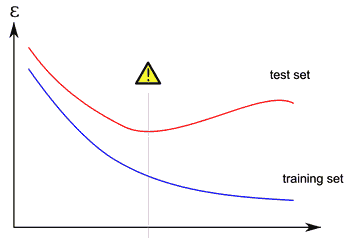
\includegraphics[width=0.4\textwidth]{Pictures/overfitting.png}
\caption{représentation du sur et sous-apprentissage}
\end{figure}
Il faut donc augmenter le nombre d'itérations et de neurones tant que les 2 courbes diminuent jusqu'à atteindre un point de la fonction entre le surapprentissage et un point où on peut encore augmenter ces paramètre, car le réseau est en sous-apprentissage.\\ \\
Une des techniques pour éviter l'overfitting est le "dropout", cette technique consiste à ignorer aléatoirement une partie des neurones à une certaine couche lors de l'apprentissage, ce qui permet de réduire la capacité du réseau à garder en mémoire les exemples. En effet, dans un réseau de neurone de type "feed forward" les neurones sont connectés à beaucoup d'autres et les neurones peuvent devenir dépendent les un des autres et ne plus fonctionner indivduellement lorsque le nombre d'epochs est grand.\cite{dropout} \footnote{cf. \url{https://medium.com/@amarbudhiraja/https-medium-com-amarbudhiraja-learning-less-to-learn-better-dropout-in-deep-machine-learning-74334da4bfc5}}\\
\begin{figure}[h]
\centering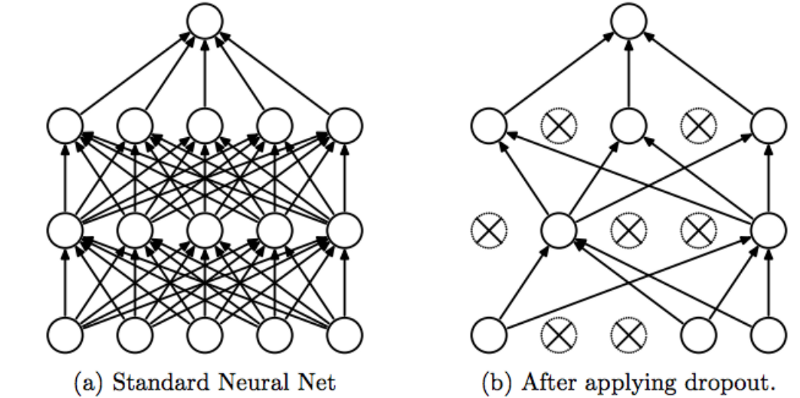
\includegraphics[width=0.6\textwidth]{Pictures/dropout.png}
\caption{différence d'un réseau avec et sans dropout, source: \url{https://medium.com/@amarbudhiraja/https-medium-com-amarbudhiraja-learning-less-to-learn-better-dropout-in-deep-machine-learning-74334da4bfc5} consulté le 13 août 2018}
\end{figure}
On remarque, sur le schéma ci-dessous(figure 3.3), que le nombre de lien est bien plus petit.\\ En conséquence, le nombre d'epochs nécessaire et plus grand mais aussi ils sont plus rapides. 
Un dropout souvent utilisé est de 0.2(on ignore 20\% des neurones), mais il convient comme avec les autre hyper-paramètres d'en tester plusieurs. Par exemple, un nombre trop élevé pour le dropout peut considérablement réduire la performance d'un réseau de neurones.\\
Cependant, le meilleur moyen de réduire l'overfitting reste d'avoir plus de data, c'est-à-dire plus d'exemples différents et variés. L'overfitting provenant de l’accoutumance du réseau à des exemples spécifique mais ne rendant pas le réseau plus performant sur le problème que le réseau doit traiter, l'overfitting peut provenir d'un manque d'exemple et surtout de variété. Ce dernier peut être commencer par une technique appelé \underline{data aumgentation}\footnote{sources : \url{https://blog.keras.io/building-powerful-image-classification-models-using-very-little-data.html}} qui consiste à transformer les données dans on dispose en les transformants légèrement(utiliser pour les CNN cf. chapitre 10)

\section{les hyper-paramètres}
Les hyper-paramètres sont les paramètres définis avant l'apprentissage(selon wikipedia)\\
Ce sont donc le nombre d'itérations, le learning rate, le biais, les fonctions d'activation ou encore le nombre de couche ou neurone par couche. Choisir les bonnes valeurs pour ses paramètres et les adapter au mesure de l'apprentissage permet de l'améliorer . Ils se différencient d'autres paramètres comme les poids des connections par le fait que ce soit l'utilisateur et non l'algorithme qui décide de leur valeur.\\ \\
Il faut donc respecter certains principes comme ne pas se baser sur l'erreur lors de l'apprentissage, c'est-à-dire se contenter d'augmenter le nombre d'itérations pour réduire l'erreur ce qui mènerait à du sur-apprentissage.\\
Tout d'abord il faut faire une liste des diffèrent hyper-paramètre à tester (varier le nombres d’itérations, activations,...)puis il faut mesurer la performance de notre modèle sur un un ensemble dit de validation pour déterminer les meilleur choix pour les hyper-paramètres. En effet, généralement nos données en environ 80\% 
pour l'apprentissage et 10\% respectivement pour la validation (mesure de performance) et le test pour mesurer la performance d'un modèle comme le perceptron ou un réseau de neurones sur une application. \cite{Hugo_Larochelle14}\\


Pour le learning rate on peut le résumer avec cette image: ,jpg
Le learnin gate est le coefficient devant le $-\nabla$ .Plus le learning rate est haut, plus l'apprentissage sera rapide. Cependant, avec un lr haut, les chances sont grandes de tomber sur un minimum local qui n'est pas le minimum absolu. C'est en effet le problème du gradient, on ne sait pas si on converge vers le minimum absolu puisqu'il nous donne uniquement la direction vers la pente décroît. \\
Ainsi, une des techniques utilisée consiste à diminuer le learning rate dans l'apprentissage si l'erreur augmente au lieu de descendre(ce qui veut dire qu'on est tombé sur le mauvais minimum). 


voir vidéo HUgo Larcohelle et pdf
\section{led types d'optimisation}
La descente de gradient stochastique n'est pas la seule méthode d'optimisation. Il en existe encore d'autre plus complexe, mais plus performantes et moins problématiques. En effet, contrairement à la descente de gradient stochastique, le taux d'apprentissage va s'adapter au cours de l'apprentissage.\\ \break 
L'algorithme \underline{AdaGrad} est une amélioration du SGD. Elle adapte les taux d'apprentissage de chaque paramètres individuellement en les rendant inversement proportionnels à la racine de la somme de la valeur au carré de tout les anciens gradients. $$ $$
LA mise à jour d'un paramètre se fait ainsi:
$$ $$\\
Adam\\
Adadelta\\
RMSprop : elle est une amélioration de l'adagrad et est une optimisation très efficace.
\url{https://keras.io/optimizers/}
%\section{soft max}
%\section {normalisation}
cf https://www.kaggle.com/yassineghouzam/introduction-to-cnn-keras-0-997-top-6 parapgraphe 2.3
\section{régularisation }
\section{data augmentation et overfitting}
Definition de overfitting: \\
Une des techniques d'optimisation pour éviter l'overfitting est le "dropout", cette technique consiste à ignorer aléatoirement une partie des neurones à une certaine pendant le training
\section{Fonctions d'activation}
Soft max, ReLu: regarder vidéo de l'indien fou\\
articles: \url{https://www.analyticsvidhya.com/blog/2017/10/fundamentals-deep-learning-activation-functions-when-to-use-them/}\\
Comme nous l'avons vu au chapitre 3.9, la fonction d'activation fait parti des hyper-paramètres. Ces fonctions ont des propriétés différentes les unes des autres et il convient donc de les connaître pour les appliquer aux problèmes appropriés.\\\\
Tout d'abord, il faut rappeler que les fonctions d'activations permettent au réseau de neurones de traiter des problèmes non-linéaires(cf. chapitre 3.1). En effet, la fonction d'activation que nous avons pour le perceptron à une couche est linéaire, car une fonction d'activation linéaire limite le réseau à ne pouvoir utiliser qu'une seule couche.\\ 
Donc les fonctions d'activation pour un réseau à plusieurs couches doivent être non-linéaire. De plus, il faut qu'elle soit dérivable en tout point, puisque la backpropagation utilise la dérivée de la fonction d'activation.\\\\ 
Il existe beaucoup de fonction d'activation, mais les plus communes sont le sigmoid que nous avons déjà présenté, la tangeant hyperbolique et ReLU(pour rectified linear unit)\\
\underline{sigmoid} était la fonction la plus utilisé aux débuts du machine learning, car son fonctionnement ressemblant aux neurones d'un cerveau est simple: la fonction renvoie un nombre entre 0 et 1 représentant le degrés d'activation d'un neurone biologique.\\
Cependant, elle a des problèmes: tout d'abord, lorsque la valeur d'un neurone s'approche de 1, le gradient devient très proche de zéros(comme on l'observe dans l'exemple 3.6) ce qui peut poser des problèmes dans certains cas, car le gradient peut disparaître(la fonction est saturée).\\
De plus, la fonction sigmoid n'est pas centré autour de zéro et peut ainsi causer des problèmes d'optimisation. En effet, avec le sigmoid, les gradients du poids sont soit tous positifs soit tous négatifs et la mise à jour peut parfois aller trop loin dans une direction ce qui ralentit l'optimisation.\\\\
Pour ces problèmes, on préfère utiliser parfois d'autre fonction d'activation. On peut cependant l'utiliser pour la dernière couche. \underline{La tangente hyperbolique} les images de cette fonction sont comprises entre 0 et 1, elle est donc centré sur 0. La fonction est : 
\[ f(x) = \frac{2}{1+\exp(-2x)}-1\]
\begin{figure}[h]
\centering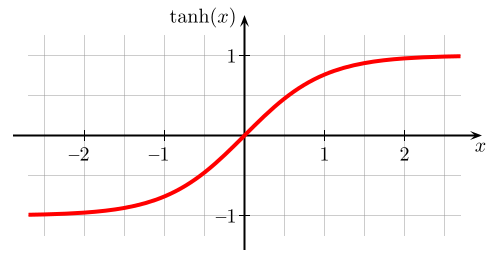
\includegraphics[width=0.6\textwidth]{Pictures/Hyperbolic_Tangent_svg.png}
\caption{représentation de la fonction tangente hyperbolique} \footnote{source:\url{https://commons.wikimedia.org/w/index.php?curid=4198479}}
\end{figure}\\
Elle a toutefois aussi le problème de disparition des gradients,néanmoins, la tangente hyperbolique devrait être utilisée au lieu du gradient.\\
La fonction \underline{ReLu} est devenu plus utilisé depuis ces dernières années. Elle s'écrit: 
\[ f(x) = max(0,x)] ou    
\begin{array}{r c l} 
AB  & = & 192 
\\C   & = & 5\,896 
\\DEF & = & 0,5
   \end{array}\]
L'image est le plus grand de 0 et de X : si X > 0: f(x) = x et si x < 0 : f(x) = 0.\\
représentation: \\
La fonction est donc linéaire à partir de 0 non-inclus. Cette propriété d'être différente à gauche et à droite l'approche de l'activation du perceptron et rend le réseau plus rapide par la simplicité de la fonction. Aussi, elle n'a pas le problème de disparition du gradient. Elle a tout de même le problème de pouvoir rendre des neurones inactifs : si le gradient d'un neurone avec ReLU est trop grand, lors de la mise à jour des poids, il se peut que ce neurone ne s'active plus du tout et le gradient avec ce neurone sera toujours de 0. Pour cela, il existe une correction de cette fonction appelé \underline{leaky ReLu} qui à une petite pente dans les négatifs ce qui fait que les poids vont continuer à se corriger, car le gradient devient un petit nombre positif. La fonction. Elle se note : 
\[f(x) =\begin{array}{r c l}
      x  &\textrm{si} & x > 0 \\
      0,001x & si & x < 0 \\
   \end{array}\]
\begin{figure}[h]
\centering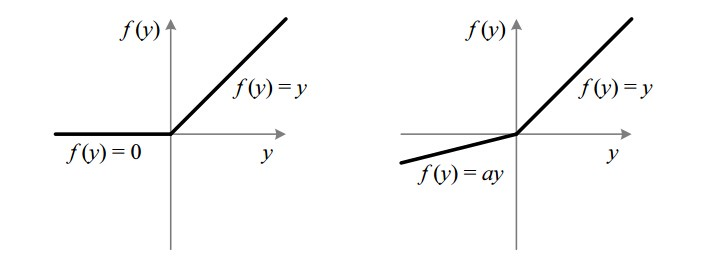
\includegraphics[width=0.6\textwidth]{Pictures/ReLu.jpeg}
\caption{représentation de la fonction ReLU à droite et leaky ReLU à gauche}
\end{figure}\\
(\underline{maxout} permet aussi de résoudre ce problème) \\ \\

C'est donc la fonction qu'on préfère utilisé au lieu du sigmoid ou de la tangent hyperbolique pour les couches caché, mais pour la couche de sortie\footnote{la couche de sortie correspond à la dernière couche, c'est-à-dire la sortie}, on utilise la fonction\underline{softmax} pour un problème de classification(qui donne une probabilité d'appartenir à une classe comme le sigmoid\footnote{à noter que la fonction sigmoid peut être utilisable pour de la classification en dernière couche}) et une fonction linéaire pour la régression puisque on ne veut pas que la valeur change.


\section{les fonctions de coût ou pertes}
%\section {epochs}
%\section{géneralisation}
\section{pandas ou comment manipuler la data(les données)}
\section{tensorflow et keras}
Tensorflow est un outil développé par google brain(section s'occupant des recherches en deep learning) pour le machine learning. Il est le framework\footnote{définition selon wikipédia : "un framework désigne un ensemble cohérent de composants logiciels structurels, qui sert à créer les fondations ainsi que les grandes lignes de tout ou d’une partie d'un logiciel (architecture).} le plus utilisé dans ce domaine. A noter qu'il en existe d'autre comme pytorch ou encore theanos.\\
L'avantage de ces librairies est leur rapidité puisque, bien que fonctionnant avec python, ils sont codé en C++ qui est un langage plus rapide(car plus proche du langage de l'ordinateur) et de plus il suffit de spécifier la structure de notre modèle et les différents paramètres au lieu d'écrire toute les formules vues ci-dessus.\\ Tensorflow contient aussi des outils permettant d'entraîner notre réseau sur un ensemble d'entraînement et ensuite d'évaluer ses performances.\\ Au lieu des matrices, on utilise une classe appelé tensor.\\
faire un MLP avec tensorflow:\\ \\
\underline{keras:}\\
Keras est un outil utilisant tensorflow permettant de définir plus facilement un réseau de neurone couche par couche. Il n'a pas autant de possibilités que avec tensorflow mais est beaucoup plus proche d'une programmation intuitive comme avec python.\\ 
exemple de MLP avec keras, cf cahier\\
Pour créer un réseau de neurone avec Keras et l'entraîner\footnote{les informations se trouvent sur le site \url{https://keras.io/}}, il y a 4 étapes fondamentales: la définitions des couches, la définition de fonction d'erreur et la méthode d'optimisation(éventuellement le taux d'apprentissage), l'entraînement et l'évaluation.\\ \\
\begin{lstlisting}
#Ajouter une couche:
model.add(Dense(output_matrix,actication= ,input shape=()))
#Dense désigne une couche où chaque neurone est connecté à chaque neurone de la couche suivante ensuite l'ordre #des éléments n'a pas d'importance, mais en général on désigne au moins le nombre de neurone, la taille de la #matrice de l'entrée(pour la 1ère couche) et l'activation.
#Après avoir définit les couches il faut compiler:
model.compile(loss= ,optimizer= )
#L'apprentissage se fait avec:
model.fit(x,yt\footnote{respectivement l'ensemble d'entraînement et le résultat visé(output target)},batch_size= ,epochs = verbose, callbacks = ,validation_split= ,validation_data = )
#Finalement, pour évaluer(c'est-à-dire tester le réseau sur un ensemble de test:
model.evalutate(x_test,y_train,...).\\ 
On peut également faire des prédiction sur des cas nouveau avec $model.predict(x\footnote{ce x représente des cas nouveau qui sont hors de l'ensemble d'entraînement},batch_size,verbose,steps).\\
exemple complet en annexe
#Séparer la data:
X_train, X_val, Y_train, Y_val = train_test_split(X_train, Y_train, test_size = 0.1)
\end{lstlisting}
Exemple en annexe

 
%\section{pytorch, theanos,...}
%\section{exemple d'apprentissage avec keras ? ou à mettre sous le chapitre keras} 
%\section{autre coût: categorical crossentropy et sparse categorical crossentropy: à mettre sous le chapitre CNN}
%\chapter{regression (PAS DE SIGMOID OU DIVISé L'INPUT OU OUTPUT POUR AVOIR DES NOMBRES ENTRE 0 ET 1}
%\section{problème du sigmoid}
%VOIR: KERAS CHEAT SHEET(en favoris)
%Regression: output dim = 1
%Il ne peut que produire un output entre et 0 et 1: ne fonctionne pas si on veut un nombre plsu grand ou plus petit.
%Cependant, on peut diviser l'ouput target (yt) pour avoir des nombres entre 0 et 1!!!!!!!!!!!!!!!!!!!!!!(ex: météo)
%\chapter{classification avec : sigmoid(probabilité d'appartenir à uen classe}
%\chapter{classification classes: crossentropy}
\chapter{deeplearning}
\chapter{prédire la météo avec le machine learning: comparaison de perforamnce avec SGD, tanh, adagrad, prendre des screenshots}
Prédire la météo est très important dans la vie humaine. Au cours de l'histoire différentes techniques plus ou moins élaborées ont existé. Cependant, malgré la technologie actuelle, les prédictions météos ne sont pas toujours justes.\\
La difficulté de cette manœuvre vient du fait que la météo est un système comparable avec l'effet papillon des films de sciences fiction. En effet, un petit changement dans l'état initial influence grandement le système : on dit qu'elle a \underline{ un comportement chaotique}. On l'étudie justement en utilisant \underline{théorie du chaos}.\\
Cependant, un réseau de neurones pourrait performer mieux que les méthodes habituelles(car l'utilisation de beaucoup de donner peut révéler des résultats parfois étonnants)ou sinon mettre en évidence la propriété chaotique de la météo.\cite{chaos}\\\\
Ce modèle utilise la régression, c'est-à-dire un réseau qui prend un ensemble de donner en entrée et renvoie un nombre en sortie. C'est le type de réseau utilisé pour faire des prédictions, par exemple, pour prédire le marché boursier.\\
Le but est d'utiliser les données de température, de précipitation, d'humidité,... des jours précédents, pris grâce à l'API du site météo wunderground, pour prédire la température moyenne d'un jour donné.\\
\cite{weather}\\
Le code se trouve en annexe.\\\\
\underline{Résultats:}
%\begin{figure}[h]
%    \centering
%    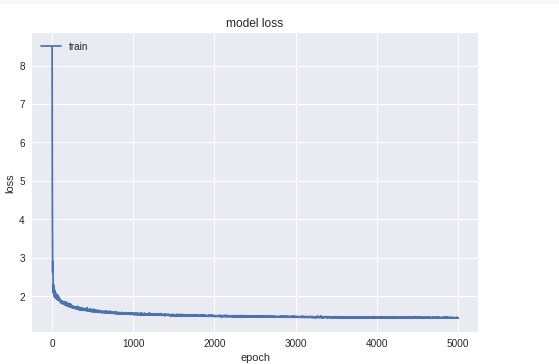
\includegraphics[width=0.3\textwidth]{Pictures/Loss weather.JPG}
%\end{figure}
\begin{figure}[h]
    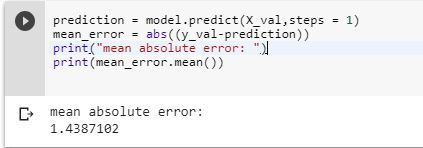
\includegraphics[width=0.5\textwidth]{Pictures/weather error.JPG}
\end{figure}


%\chapter{projet de classifcation avec reconnaissance d'image}
\chapter{Les CNN(convolutional neural network)}
\section{principes}
Un CNN est un type de réseau de neurone utilisé pour la reconnaissance d'image, mais son utilisation peut être large comme apprendre à jouer à jeu par la reconnaissance de patterns ou même reconnaître des sons en utilisant l'intensité des fréquences de sons à travers le temps(ce qui forme un quadrillage comme pour les images) ainsi que pour du texte\footnote{on peut utiliser ces réseaux pour tout types de données transformable en une sorte d'image avec des pattern et des features}. Ils sont construits de plusieurs couches spécifiques et les neurones représentent des parties distinctives\footnote{ces parties distinctifs sont mathématiquement une combinaisons de pixels qui reviennent d'une image à l'autre} d'une image que le réseau à détecté comme des yeux pour un visage et des roues pour une voiture. Pour distinguer une roue, le même principe s'applique : l'algorithme recherche des éléments qui reviennent comme une boucle, un rond, un trait. En définitif, il décompose l'image en différentes parties. Ce processus permet de désigner comme roue plusieurs images de roues différentes.\\ \\
\section{convolution}
La première étape est de transformer les images en une matrice à 2 dimensions contenant les niveaux de gris des pixels ce qui permet de transformer le problème en un problème mathématique qu'un ordinateur peut comprendre. L'image devient un ensemble de carrés(pixels) ayant chacun un nombre correspondant à leur niveau de gris\footnote{le niveau de gris représente la luminostié d'un pixel\url{https://fr.wikipedia.org/wiki/Niveau_de_gris}} par exemple un pixel blanc aura la valeur 1 et un pixel noir 0.\\
Alors ce qu'on a désigner plus haut comme "bout d'image" appelé \underline{"features"} sont en fait une combinaison de pixel de valeur similaire comme  une diagonale, un trait ou une boucle par exemple. Le but pour le réseau est de trouver ces features et ensuite de les utiliser pour mettre en lien des images. Le processus permettant de retrouver une feature
sur une autre image s'appelle mathématiquement le \underline{"filtering"}. Il se compose de 4 étapes : tout d'abord aligner une feature avec une partie de l'image à analyser, ensuite multiplier la valeur des pixels de ce dernier avec ceux de la feature, les additionner et diviser par le nombre total dans la feature. \\
\begin{figure}[h]
\centering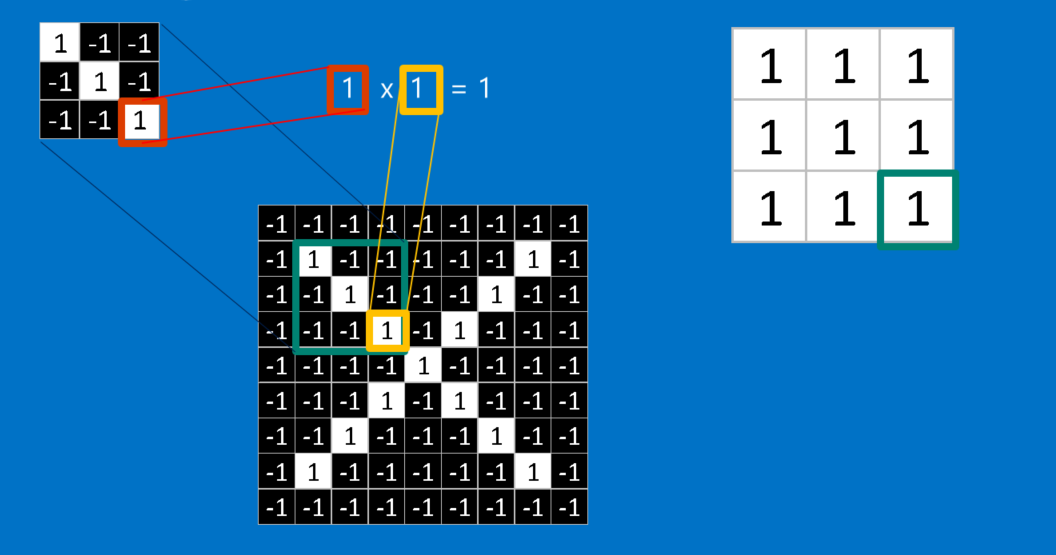
\includegraphics[width=0.4\textwidth]{Pictures/cnn5.png}
\caption{exemple de filtering source:\url{http://brohrer.github.io/how_convolutional_neural_networks_work.html}}
\end{figure}
Sur l'exemple ci- dessus le calcul donne:
\[\frac{1+1-1+1+1+1-1+1+1}{9} = 0,55 \]
Cette valeur montre à quel point la feature est le bout d'image correspondent. L'algorithme va bouger le filtre à travers l'image et répéter ces étapes pour retrouver la feature sur l'image en question ce qui va donner au finale une grille avec différentes valeurs permettant de voir si on retrouve une forme sur l'image.\\
\begin{figure}[h]
\centering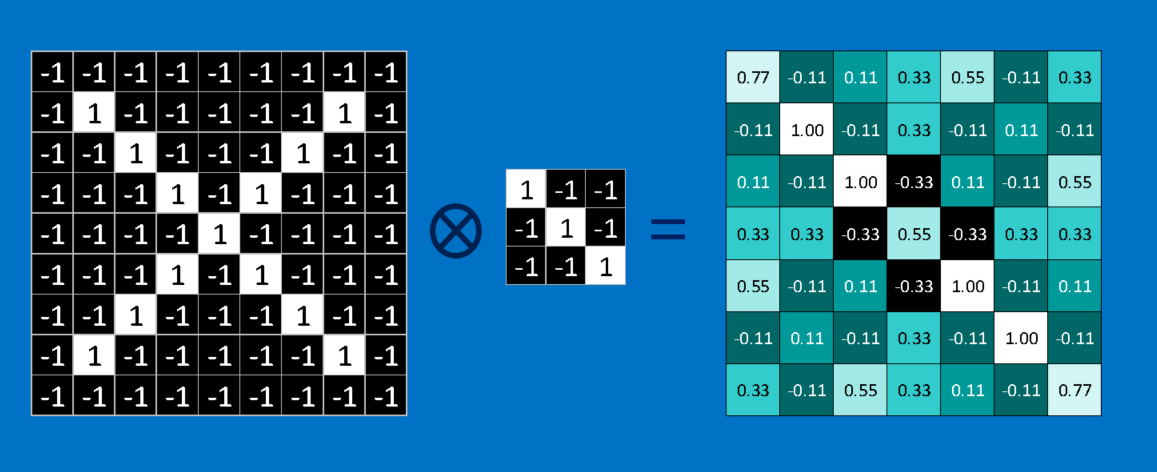
\includegraphics[width=0.6\textwidth]{Pictures/cnn6__1_.png}
\caption{exemple de convolution source:\url{http://brohrer.github.io/how_convolutional_neural_networks_work.html}}
\end{figure}
Ce processus de bouger le filtre pour retrouver les features s'appelle \underline{convolution}.
Cette grille montre où la feature apparaît. En effet, les valeurs sont élevés où la diagonale apparaît.\\
Le but d'une \underline{couche de convolution} est de répéter cette convolution avec les différents features pour obtenir différentes images filtrées. \underline{C'est la transformation d'une image en une pile d'image filtrées}. Ce type de couche est le premier élément essentiel d'un CNN.\\
\section{couche de pooling}
Le 2ème type de couche spécifique aux réseaux neuronaux convolutifs est la pooling layer, elle suit directement la convolution. Le but est de diminuer la pile d'image créée pour chaque features. Pour ce faire il faut prendre un cadre de 2x2 ou 3x3 et un nombre de case à avancer(normalement 2). Le but est de déplace le cadre de 2 pixels et à chaque fois de répertorier sur une 2ème grille plus petite la valeur la plus grande dans notre. En se déplaçant ainsi à travers la première grille, on obtient une 2ème grille plus petite, mais on y retrouve toujours les features avec les hautes valeurs.\\ Avec cette opération, la taille de l'image diminue par 2, ce qui est nécessaire car les images ont souvent plusieurs millier de pixels en taille. De plus, le pooling permet de retrouver toute les features, car le cadre sélectionne la valeur la plus haute, ce qui fait que la position ne sera pas un problème.\\
La 3ème technique utilisé pour ces réseaux est la  \underline{normalisation}. Comme lorsqu'on norme un vecteur, on change les valeurs pour qu'elles soient tous comprises entre 0 et 1. Pour cela, on passe les valeurs des pixels à travers la fonction ReLU.\footnote{ chapitre sur les fonctions d'activation}Avec cette fonction, les nombre négatifs vont se transformer en zéros.\\
L'ordre des opérations d'un CNN est donc une couche convolutif avec ReLu et le pooling à travers lesquels on passe une matrice. Cependant, on peut faire des réseaux plus grands(deep learning) et répéter les différentes étapes. C'est ce qu'on appelle le \underline{deep stacking}: on peut par exemple effectuer 2 convolutions de suite, puis un pooling, puis à nouveau une convolutions etc...
\begin{figure}[h]
\centering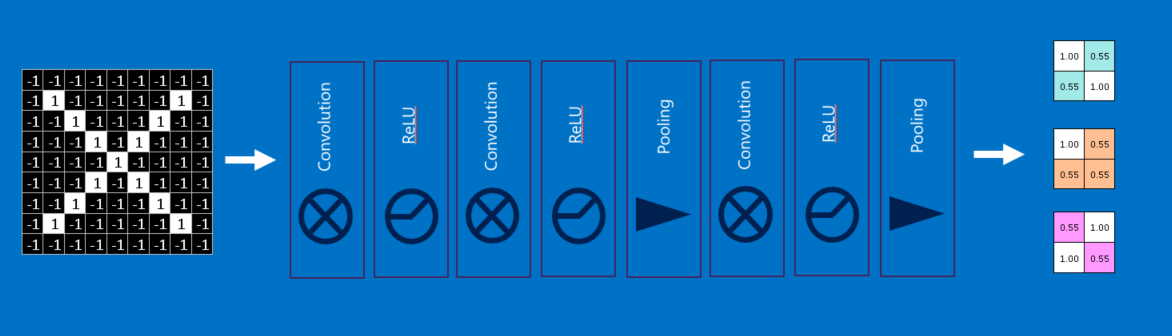
\includegraphics[width=0.6\textwidth]{Pictures/cnn12__1_.png}
\caption{exemple de deep stacking source:\url{http://brohrer.github.io/how_convolutional_neural_networks_work.html}}
\end{figure}
Après ces modifications, notre pile d'image est beaucoup plus petite ce qui fait que les features sont de plus en plus nombreuses et précise.\\
\section{dernières couches d'un CNN}
Enfin,la dernière couche d'un CNN est appelée \underline{une couche entièrement connectée}\footnote{
fully connected layer en anglais}. A cette étape, on retrouve le même principe que les liaisons des réseaux de neurones vu jusqu'à présent. La sortie du réseau est une image à reconnaître comme des chiffres et les processus d'avant nous ont permis de séparer les images à analyser en éléments. Dans cette couche, les poids des connections d'une image et d'une features de cette image sont plus élevés; c'est la fameuse règle de Hebb:« des neurones qui s'excitent ensemble se lient entre eux. » (« cells that fire together, wire together »).\\
On peut symboliser cette opération par un vote: chaque valeur de notre pile de grille vote par rapport à l'image finale qui leur correspond et les votes(connections) ont plus de poids si une valeur prédit telle ou telle image. Par exemple, une connexion reliant une feature en courbe et le chiffre 8 a plus de poids que cette features relié au chiffre 1.\\
Ainsi, les valeurs des neurones par rapport aux poids des connections, permettent de prédire, de faire une hypothèse\footnote{cette hypothèse peut être vue comme une probabilité d'appartenir à une classe comme pour les perceptrons} comme pour les perceptron et l'écart entre ce qui est prédit et ce qui est ciblé, à savoir la vraie image correspondant à l'entrée, nous permet de corriger les paramètres avec la backpropagation.\\
Ainsi, à partir de cette étape, le réseau fonctionne de la même façon que les réseaux vus ci-dessus donc on peut tout à fait avoir plusieurs couches avec des couches cachées après les couches convolutifs et de pooling.\\
\section{les hyper-paramètres d'un CNN}
On retrouve les même hyper-paramètre que ceux vu précédemment(activation,biais,nombre de couches cachées,...), mais il y en aussi de nouvelle avec l'ajout des couches convolutifs et de pooling.\\
Avec ces couches, il faut prendre en compte le nombre de features, la taille des features pour la convolution et la taille du cadre et le nombre nombre de pixel auquel avance le cadre.
%\section{autre coût: categorical crossentropy et sparse categorical crossentropy}
%C'est une fonction d'erreur spécifique à une classification de plus de 2 classes. Le principe est le même %: différence entre l'hypothèse et réponse. Il existe toutefois une version de ce coût pour 2 classes %appelé binary crossentropy


%Normaliser comme pour les vecteur : avoir un nombre entre 0 et 1, utile pour le grayscale car %l'apprentissage se fait plus rapidement.\\
%former les classe, labelliser\\
sources:
\url{https://www.kaggle.com/yassineghouzam/introduction-to-cnn-keras-0-997-top-6}\\
\url{https://www.youtube.com/watch?v=FmpDIaiMIeA}
\section{exemple de reconnaisance avec cifar10}
L'ensemble d'image cifar-10 est très utilisé pour tester des réseaux CNN. Il regroupe 60'000 images 32x32 en couleur; parmi celles-ci, il y a respectivement 6'000 images d'avions, voitures, oiseaux, chats, cerfs, chiens, grenouille, chevaux, bateaux et camions\footnote{à noter qu'il existe une version avec 100 type d'images(cifar-100}.\\
Le réseau utilisé est un deep CNN avec 3x[2x(Conv2D+relu)+pooling] ce qui permet d'obtenir 85\% accuracy.\\
\begin{figure}[h]
\centering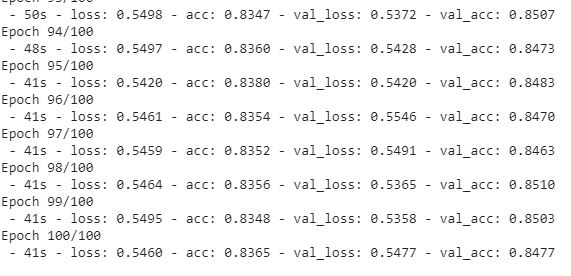
\includegraphics[width=0.6\textwidth]{Cifar-10.JPG}
\caption{résultat du CNN} 
\end{figure}\\
Certains réseau arrive à obtenir 95\%+ d'accuracy 





%\chapter{RNN(recursive...)}
%\chapter{GAN, WGAN}
\chapter{Ml et marketing,journal,...}
\printbibliography[title=Sources]

%\bibliographystyle{IEEEtran}
%\bibliography{bibliography.bib}


%\nocite{*}
%\printbibheading[title={Publications}]
%\printbibliography[nottype=online,heading=subbibliography,
%title={Printed Sources},resetnumbers=true]
%\printbibliography[type=online,heading=subbibliography,
%title={Online Sources},resetnumbers=true]

\end{document}